\documentclass[twoside]{book}

% Packages required by doxygen
\usepackage{fixltx2e}
\usepackage{calc}
\usepackage{doxygen}
\usepackage[export]{adjustbox} % also loads graphicx
\usepackage{graphicx}
\usepackage[utf8]{inputenc}
\usepackage{makeidx}
\usepackage{multicol}
\usepackage{multirow}
\PassOptionsToPackage{warn}{textcomp}
\usepackage{textcomp}
\usepackage[nointegrals]{wasysym}
\usepackage[table]{xcolor}

% Font selection
\usepackage[T1]{fontenc}
\usepackage[scaled=.90]{helvet}
\usepackage{courier}
\usepackage{amssymb}
\usepackage{sectsty}
\renewcommand{\familydefault}{\sfdefault}
\allsectionsfont{%
  \fontseries{bc}\selectfont%
  \color{darkgray}%
}
\renewcommand{\DoxyLabelFont}{%
  \fontseries{bc}\selectfont%
  \color{darkgray}%
}
\newcommand{\+}{\discretionary{\mbox{\scriptsize$\hookleftarrow$}}{}{}}

% Page & text layout
\usepackage{geometry}
\geometry{%
  a4paper,%
  top=2.5cm,%
  bottom=2.5cm,%
  left=2.5cm,%
  right=2.5cm%
}
\tolerance=750
\hfuzz=15pt
\hbadness=750
\setlength{\emergencystretch}{15pt}
\setlength{\parindent}{0cm}
\setlength{\parskip}{0.2cm}
\makeatletter
\renewcommand{\paragraph}{%
  \@startsection{paragraph}{4}{0ex}{-1.0ex}{1.0ex}{%
    \normalfont\normalsize\bfseries\SS@parafont%
  }%
}
\renewcommand{\subparagraph}{%
  \@startsection{subparagraph}{5}{0ex}{-1.0ex}{1.0ex}{%
    \normalfont\normalsize\bfseries\SS@subparafont%
  }%
}
\makeatother

% Headers & footers
\usepackage{fancyhdr}
\pagestyle{fancyplain}
\fancyhead[LE]{\fancyplain{}{\bfseries\thepage}}
\fancyhead[CE]{\fancyplain{}{}}
\fancyhead[RE]{\fancyplain{}{\bfseries\leftmark}}
\fancyhead[LO]{\fancyplain{}{\bfseries\rightmark}}
\fancyhead[CO]{\fancyplain{}{}}
\fancyhead[RO]{\fancyplain{}{\bfseries\thepage}}
\fancyfoot[LE]{\fancyplain{}{}}
\fancyfoot[CE]{\fancyplain{}{}}
\fancyfoot[RE]{\fancyplain{}{\bfseries\scriptsize Generated on Wed Feb 25 2015 17\+:32\+:06 for Yap by Doxygen }}
\fancyfoot[LO]{\fancyplain{}{\bfseries\scriptsize Generated on Wed Feb 25 2015 17\+:32\+:06 for Yap by Doxygen }}
\fancyfoot[CO]{\fancyplain{}{}}
\fancyfoot[RO]{\fancyplain{}{}}
\renewcommand{\footrulewidth}{0.4pt}
\renewcommand{\chaptermark}[1]{%
  \markboth{#1}{}%
}
\renewcommand{\sectionmark}[1]{%
  \markright{\thesection\ #1}%
}

% Indices & bibliography
\usepackage{natbib}
\usepackage[titles]{tocloft}
\setcounter{tocdepth}{3}
\setcounter{secnumdepth}{5}
\makeindex

% Hyperlinks (required, but should be loaded last)
\usepackage{ifpdf}
\ifpdf
  \usepackage[pdftex,pagebackref=true]{hyperref}
\else
  \usepackage[ps2pdf,pagebackref=true]{hyperref}
\fi
\hypersetup{%
  colorlinks=true,%
  linkcolor=blue,%
  citecolor=blue,%
  unicode%
}

% Custom commands
\newcommand{\clearemptydoublepage}{%
  \newpage{\pagestyle{empty}\cleardoublepage}%
}


%===== C O N T E N T S =====

\begin{document}

% Titlepage & ToC
\hypersetup{pageanchor=false,
             bookmarks=true,
             bookmarksnumbered=true,
             pdfencoding=unicode
            }
\pagenumbering{roman}
\begin{titlepage}
\vspace*{7cm}
\begin{center}%
{\Large Yap }\\
\vspace*{1cm}
{\large Generated by Doxygen 1.8.9.1}\\
\vspace*{0.5cm}
{\small Wed Feb 25 2015 17:32:06}\\
\end{center}
\end{titlepage}
\clearemptydoublepage
\tableofcontents
\clearemptydoublepage
\pagenumbering{arabic}
\hypersetup{pageanchor=true}

%--- Begin generated contents ---
\chapter{Hierarchical Index}
\section{Class Hierarchy}
This inheritance list is sorted roughly, but not completely, alphabetically\+:\begin{DoxyCompactList}
\item \contentsline{section}{Actor}{\pageref{classActor}}{}
\begin{DoxyCompactList}
\item \contentsline{section}{Sprite}{\pageref{classSprite}}{}
\begin{DoxyCompactList}
\item \contentsline{section}{Player}{\pageref{classPlayer}}{}
\end{DoxyCompactList}
\end{DoxyCompactList}
\item \contentsline{section}{Grid$<$ Element $>$}{\pageref{classGrid}}{}
\item \contentsline{section}{Input}{\pageref{classInput}}{}
\begin{DoxyCompactList}
\item \contentsline{section}{Sprite}{\pageref{classSprite}}{}
\end{DoxyCompactList}
\item \contentsline{section}{Menu}{\pageref{classMenu}}{}
\item \contentsline{section}{Text}{\pageref{classText}}{}
\item \contentsline{section}{Texture}{\pageref{classTexture}}{}
\begin{DoxyCompactList}
\item \contentsline{section}{Button}{\pageref{classButton}}{}
\item \contentsline{section}{Sprite}{\pageref{classSprite}}{}
\item \contentsline{section}{ui\+Window}{\pageref{classuiWindow}}{}
\end{DoxyCompactList}
\item \contentsline{section}{Velocity}{\pageref{classVelocity}}{}
\item \contentsline{section}{Window}{\pageref{classWindow}}{}
\begin{DoxyCompactList}
\item \contentsline{section}{My\+Game\+Window}{\pageref{classMyGameWindow}}{}
\end{DoxyCompactList}
\item \contentsline{section}{World}{\pageref{classWorld}}{}
\end{DoxyCompactList}

\chapter{Class Index}
\section{Class List}
Here are the classes, structs, unions and interfaces with brief descriptions\+:\begin{DoxyCompactList}
\item\contentsline{section}{\hyperlink{classActor}{Actor} }{\pageref{classActor}}{}
\item\contentsline{section}{\hyperlink{classButton}{Button} }{\pageref{classButton}}{}
\item\contentsline{section}{\hyperlink{classGrid}{Grid$<$ Element $>$} }{\pageref{classGrid}}{}
\item\contentsline{section}{\hyperlink{classInput}{Input} }{\pageref{classInput}}{}
\item\contentsline{section}{\hyperlink{classMenu}{Menu} }{\pageref{classMenu}}{}
\item\contentsline{section}{\hyperlink{classMyGameWindow}{My\+Game\+Window} }{\pageref{classMyGameWindow}}{}
\item\contentsline{section}{\hyperlink{classPlayer}{Player} }{\pageref{classPlayer}}{}
\item\contentsline{section}{\hyperlink{classSprite}{Sprite} }{\pageref{classSprite}}{}
\item\contentsline{section}{\hyperlink{classText}{Text} }{\pageref{classText}}{}
\item\contentsline{section}{\hyperlink{classTexture}{Texture} }{\pageref{classTexture}}{}
\item\contentsline{section}{\hyperlink{classuiWindow}{ui\+Window} }{\pageref{classuiWindow}}{}
\item\contentsline{section}{\hyperlink{classVelocity}{Velocity} }{\pageref{classVelocity}}{}
\item\contentsline{section}{\hyperlink{classWindow}{Window} }{\pageref{classWindow}}{}
\item\contentsline{section}{\hyperlink{classWorld}{World} }{\pageref{classWorld}}{}
\end{DoxyCompactList}

\chapter{Class Documentation}
\hypertarget{classActor}{}\section{Actor Class Reference}
\label{classActor}\index{Actor@{Actor}}
Inheritance diagram for Actor\+:\begin{figure}[H]
\begin{center}
\leavevmode
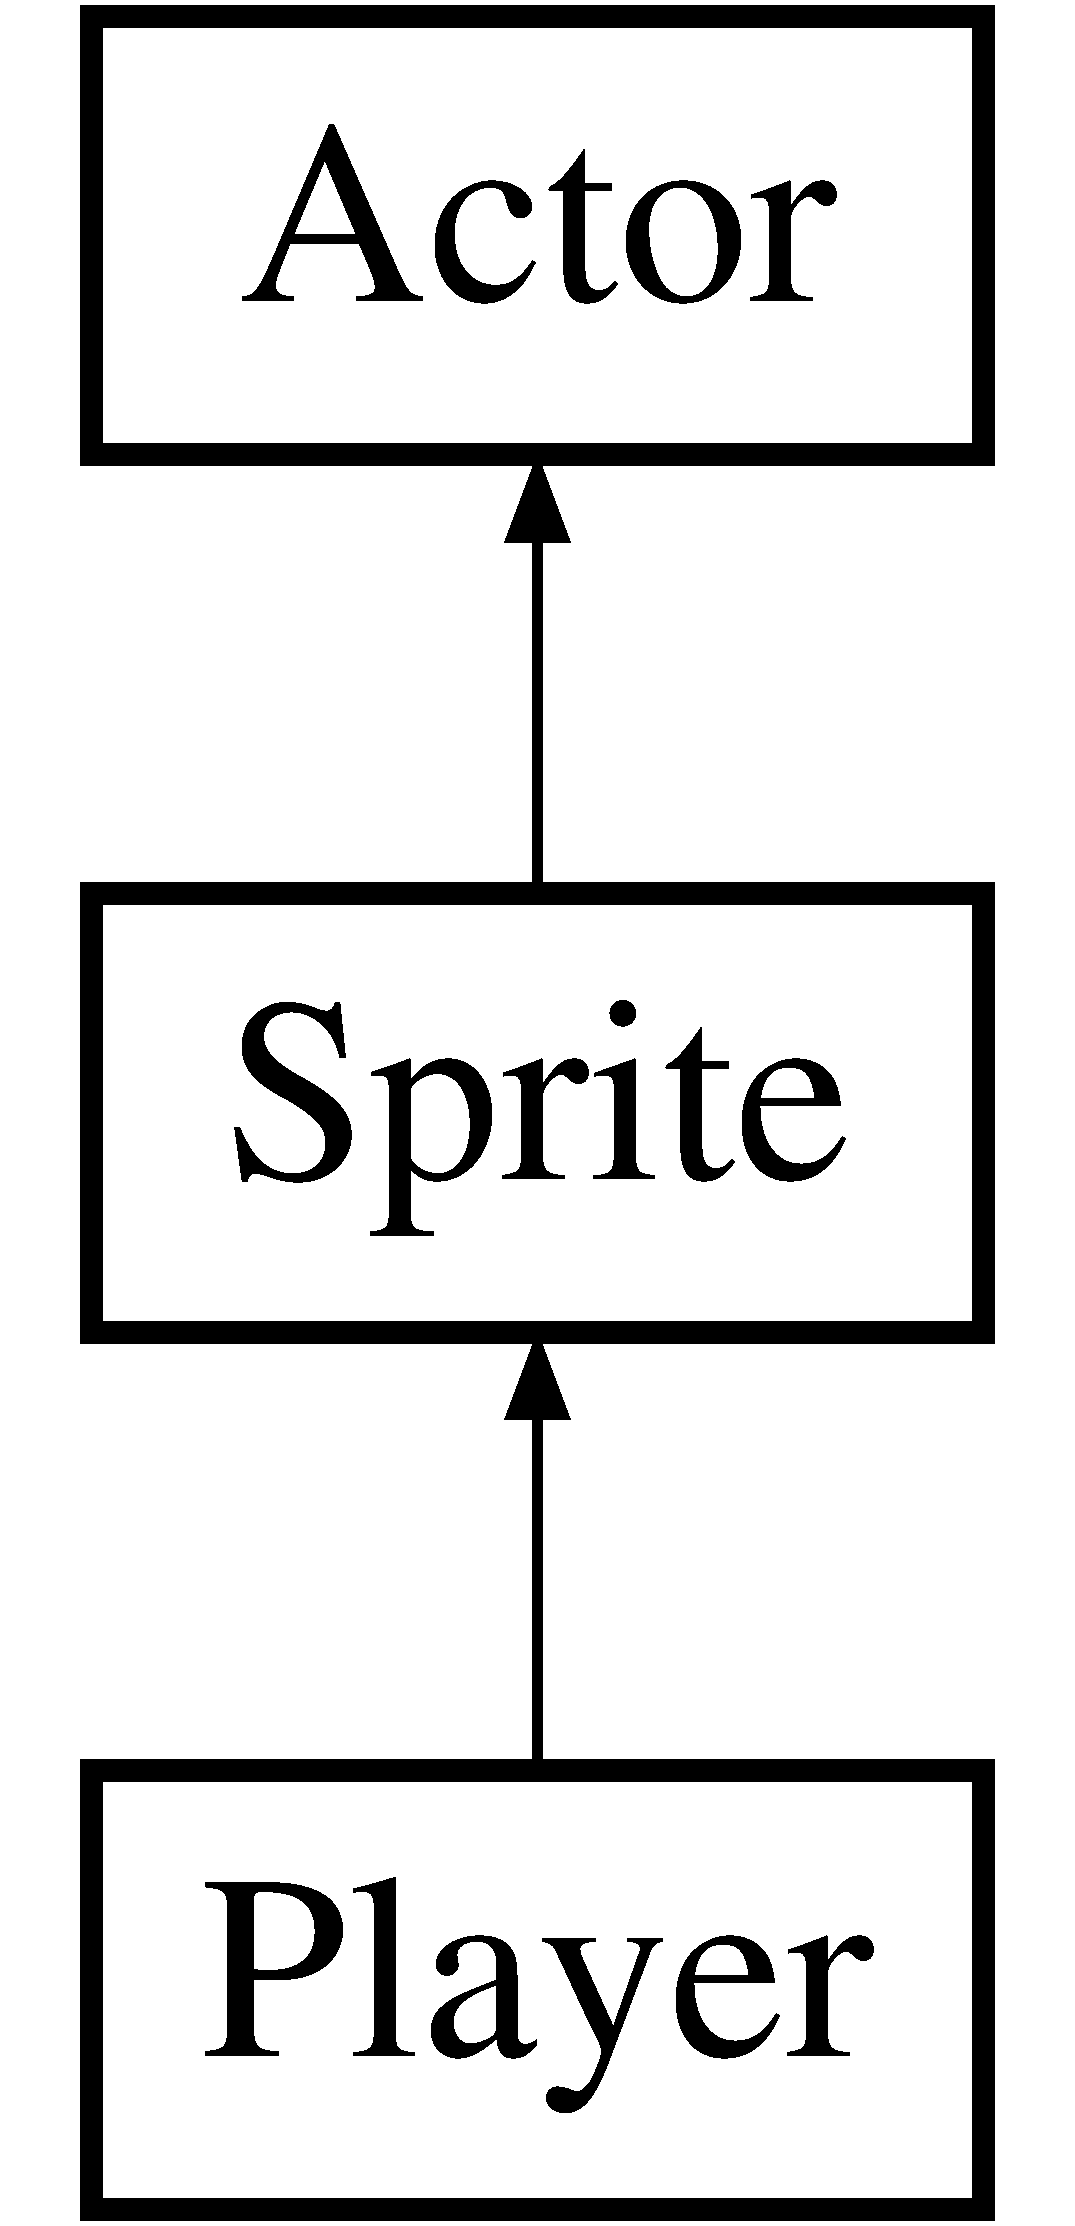
\includegraphics[height=3.000000cm]{classActor}
\end{center}
\end{figure}
\subsection*{Public Member Functions}
\begin{DoxyCompactItemize}
\item 
\hypertarget{classActor_ae9a45ebaba49b13249c0edfa4bf1e2bb}{}{\bfseries Actor} (cp\+Vect pos, cp\+Vect sz, bool is\+Dynamic)\label{classActor_ae9a45ebaba49b13249c0edfa4bf1e2bb}

\item 
\hypertarget{classActor_abc8d269860882fc2832fbfa85d632f20}{}void {\bfseries set\+Density} (float density)\label{classActor_abc8d269860882fc2832fbfa85d632f20}

\item 
\hypertarget{classActor_a7c3ae89083445a199cbdf27194e91dc0}{}void {\bfseries set\+Friction} (float friction)\label{classActor_a7c3ae89083445a199cbdf27194e91dc0}

\item 
\hypertarget{classActor_abb65c8d326472d93b852236685976e12}{}void {\bfseries create\+Box} (\hyperlink{classWorld}{World} w, cp\+Vect pos, cp\+Float mass, cp\+Float moment, S\+D\+L\+\_\+\+Rect Size)\label{classActor_abb65c8d326472d93b852236685976e12}

\item 
\hypertarget{classActor_af10d6f5b2ce4f5ab7a43c813b8b5bf95}{}void {\bfseries update} ()\label{classActor_af10d6f5b2ce4f5ab7a43c813b8b5bf95}

\item 
\hypertarget{classActor_a6bc4555f1e1f649cea66e87f1c283cc3}{}cp\+Body $\ast$ {\bfseries get\+Body} ()\label{classActor_a6bc4555f1e1f649cea66e87f1c283cc3}

\item 
\hypertarget{classActor_a07b5f28631e5f62963657c672e9c8449}{}void {\bfseries move} (cp\+Vect pos)\label{classActor_a07b5f28631e5f62963657c672e9c8449}

\end{DoxyCompactItemize}
\subsection*{Public Attributes}
\begin{DoxyCompactItemize}
\item 
\hypertarget{classActor_af6ad7b874a6cef5291367e149d7683c4}{}cp\+Vect {\bfseries position}\label{classActor_af6ad7b874a6cef5291367e149d7683c4}

\item 
\hypertarget{classActor_aec6e9e96e6edf0f712394ed1596a65a6}{}cp\+Vect {\bfseries velocity}\label{classActor_aec6e9e96e6edf0f712394ed1596a65a6}

\item 
\hypertarget{classActor_a85abf21455f366fdc4ed38288bbcc9b2}{}cp\+Body $\ast$ {\bfseries body}\label{classActor_a85abf21455f366fdc4ed38288bbcc9b2}

\item 
\hypertarget{classActor_a80dd1c1a1ebba5b41082ac00ff1af131}{}cp\+Shape $\ast$ {\bfseries shape}\label{classActor_a80dd1c1a1ebba5b41082ac00ff1af131}

\item 
\hypertarget{classActor_a886708bf688a5253b1fc8191b630c0ae}{}cp\+Vect {\bfseries size}\label{classActor_a886708bf688a5253b1fc8191b630c0ae}

\item 
\hypertarget{classActor_aadf37d2c3d3123cc9b60f79e0fe11530}{}cp\+Float {\bfseries radius}\label{classActor_aadf37d2c3d3123cc9b60f79e0fe11530}

\item 
\hypertarget{classActor_a7cf3ec4b52eb243377cdcdc3908f6deb}{}bool {\bfseries dynamic}\label{classActor_a7cf3ec4b52eb243377cdcdc3908f6deb}

\end{DoxyCompactItemize}


The documentation for this class was generated from the following file\+:\begin{DoxyCompactItemize}
\item 
/home/batman/code/my\+\_\+git\+\_\+code/yap/src/physics/actor.\+hpp\end{DoxyCompactItemize}

\hypertarget{classButton}{}\section{Button Class Reference}
\label{classButton}\index{Button@{Button}}
Inheritance diagram for Button\+:\begin{figure}[H]
\begin{center}
\leavevmode
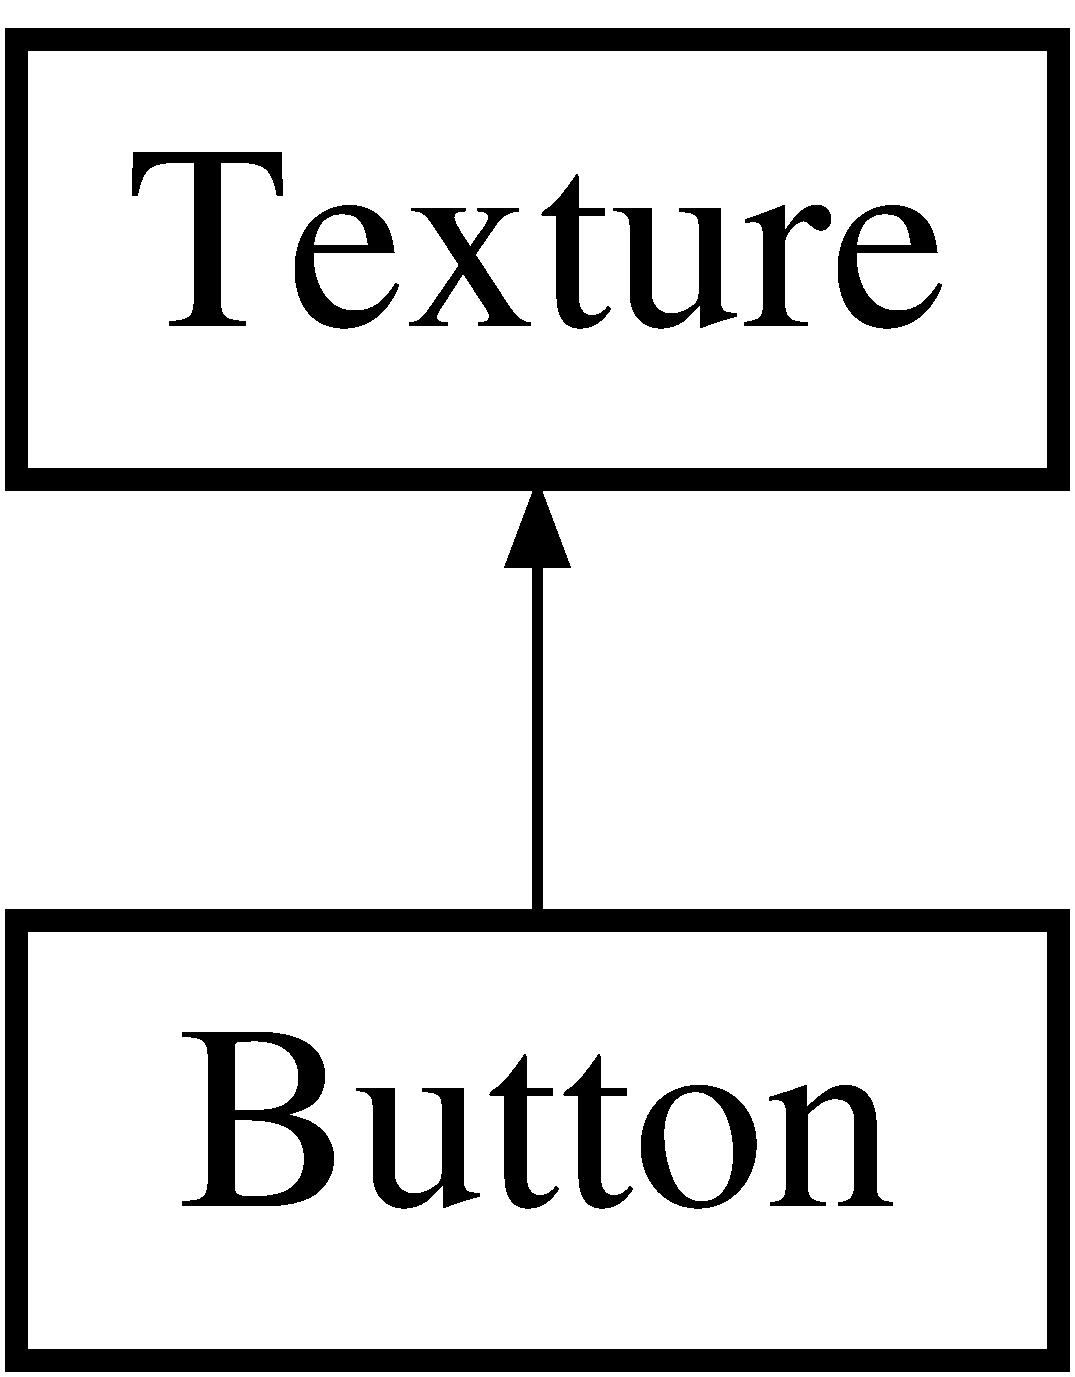
\includegraphics[height=2.000000cm]{classButton}
\end{center}
\end{figure}
\subsection*{Public Member Functions}
\begin{DoxyCompactItemize}
\item 
\hypertarget{classButton_abe0413b847c42db7181f0ca54c3606d5}{}{\bfseries Button} (std\+::string texname, int x, int y, S\+D\+L\+\_\+\+Renderer $\ast$rnd, S\+D\+L\+\_\+\+Window $\ast$window)\label{classButton_abe0413b847c42db7181f0ca54c3606d5}

\item 
\hypertarget{classButton_a168e3e56188d3f5166e983fbbe9dd95f}{}void {\bfseries on\+Click} (int x, int y, std\+::function$<$ void(S\+D\+L\+\_\+\+Renderer $\ast$rnd, S\+D\+L\+\_\+\+Event \&event, S\+D\+L\+\_\+\+Window $\ast$window)$>$ callback, S\+D\+L\+\_\+\+Renderer $\ast$rnd, S\+D\+L\+\_\+\+Event \&event, S\+D\+L\+\_\+\+Window $\ast$window)\label{classButton_a168e3e56188d3f5166e983fbbe9dd95f}

\end{DoxyCompactItemize}
\subsection*{Protected Attributes}
\begin{DoxyCompactItemize}
\item 
\hypertarget{classButton_a34c86ea937a95ea66c4a0a60e08b4ae8}{}S\+D\+L\+\_\+\+Rect $\ast$ {\bfseries bounds}\label{classButton_a34c86ea937a95ea66c4a0a60e08b4ae8}

\end{DoxyCompactItemize}


The documentation for this class was generated from the following file\+:\begin{DoxyCompactItemize}
\item 
/home/batman/code/my\+\_\+git\+\_\+code/yap/src/gfx/ui/button.\+hpp\end{DoxyCompactItemize}

\hypertarget{classGrid}{}\section{Grid$<$ Element $>$ Class Template Reference}
\label{classGrid}\index{Grid$<$ Element $>$@{Grid$<$ Element $>$}}
\subsection*{Public Member Functions}
\begin{DoxyCompactItemize}
\item 
\hypertarget{classGrid_a9d6473a70d115ce68b14449e89b80435}{}{\bfseries Grid} (int x=0, int y=0, int p=50, int gw=3, int gh=3)\label{classGrid_a9d6473a70d115ce68b14449e89b80435}

\item 
\hypertarget{classGrid_ace1892d9c1c042ec34d3339d1736b5ff}{}void {\bfseries gridify} ()\label{classGrid_ace1892d9c1c042ec34d3339d1736b5ff}

\item 
\hypertarget{classGrid_a72b63b1c76b2132de2d333205a492356}{}void {\bfseries update} ()\label{classGrid_a72b63b1c76b2132de2d333205a492356}

\item 
\hypertarget{classGrid_a61404b16f274eae8be51b3471774f68e}{}void {\bfseries append} (Element \&element)\label{classGrid_a61404b16f274eae8be51b3471774f68e}

\end{DoxyCompactItemize}
\subsection*{Protected Attributes}
\begin{DoxyCompactItemize}
\item 
\hypertarget{classGrid_a0185fd7d0762d902e272d9ce10641a20}{}std\+::vector$<$ Element $>$ {\bfseries grid}\label{classGrid_a0185fd7d0762d902e272d9ce10641a20}

\item 
\hypertarget{classGrid_a823547c352ccd94d75b16adfb8bbb564}{}int {\bfseries padding}\label{classGrid_a823547c352ccd94d75b16adfb8bbb564}

\item 
\hypertarget{classGrid_a08f873f5d1b6e540beb79d63cca07b6a}{}int {\bfseries gx}\label{classGrid_a08f873f5d1b6e540beb79d63cca07b6a}

\item 
\hypertarget{classGrid_a702d5995bed02313afca00ff6e7dc390}{}int {\bfseries gy}\label{classGrid_a702d5995bed02313afca00ff6e7dc390}

\item 
\hypertarget{classGrid_a56594934f91fa3426b0ea22451ede533}{}S\+D\+L\+\_\+\+Rect {\bfseries position}\label{classGrid_a56594934f91fa3426b0ea22451ede533}

\end{DoxyCompactItemize}


The documentation for this class was generated from the following file\+:\begin{DoxyCompactItemize}
\item 
/home/batman/code/my\+\_\+git\+\_\+code/yap/src/gfx/ui/grid.\+hpp\end{DoxyCompactItemize}

\hypertarget{classInput}{}\section{Input Class Reference}
\label{classInput}\index{Input@{Input}}
Inheritance diagram for Input\+:\begin{figure}[H]
\begin{center}
\leavevmode
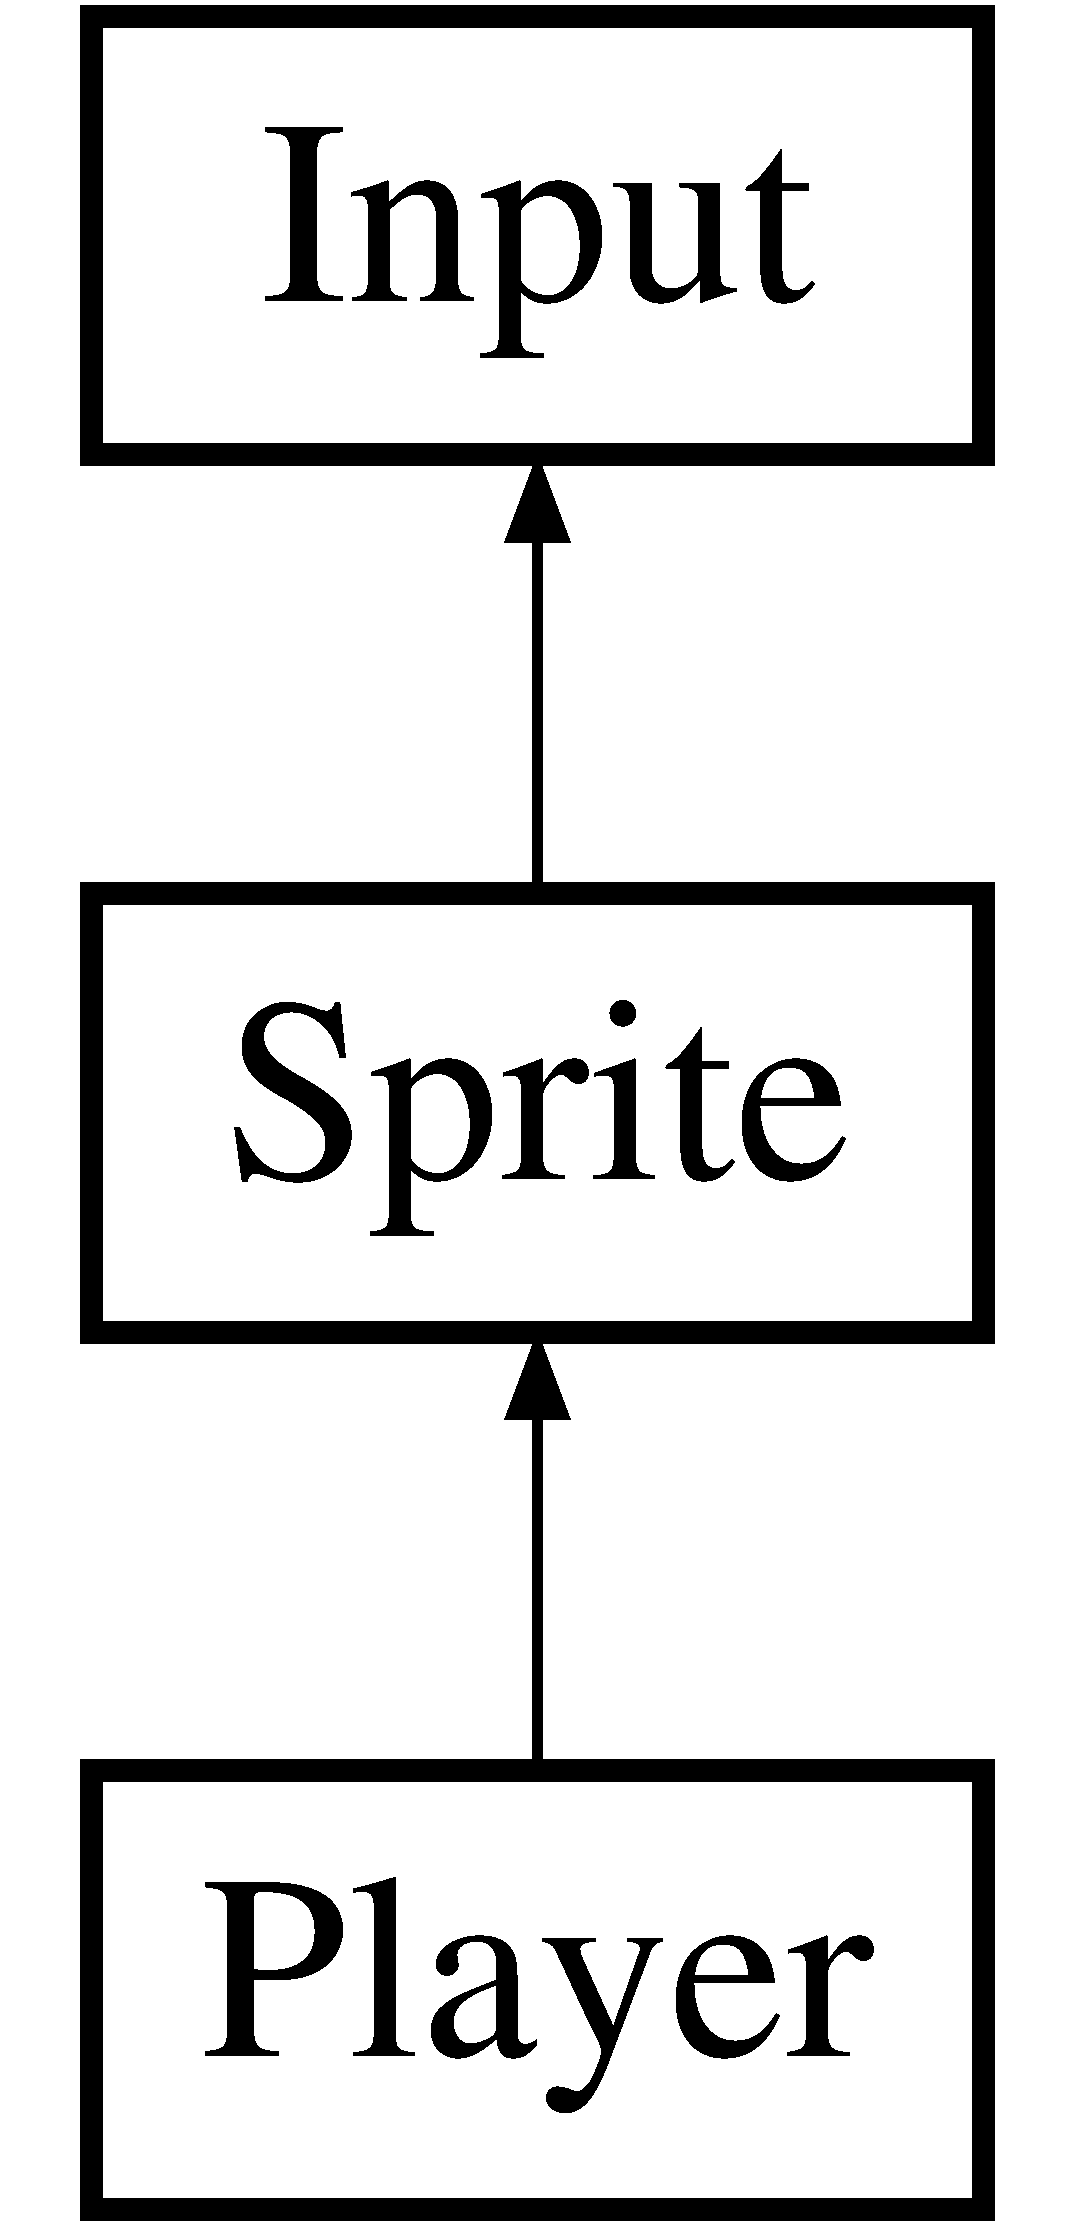
\includegraphics[height=3.000000cm]{classInput}
\end{center}
\end{figure}
\subsection*{Public Member Functions}
\begin{DoxyCompactItemize}
\item 
\hypertarget{classInput_adff580a5ada93ea9d1e95f8e7da4ba0d}{}virtual void {\bfseries handle\+Events} ()\label{classInput_adff580a5ada93ea9d1e95f8e7da4ba0d}

\item 
\hypertarget{classInput_aa05b96592a3283e2ddce503417db0bee}{}{\bfseries Input} (S\+D\+L\+\_\+\+Event \&ev)\label{classInput_aa05b96592a3283e2ddce503417db0bee}

\end{DoxyCompactItemize}
\subsection*{Protected Attributes}
\begin{DoxyCompactItemize}
\item 
\hypertarget{classInput_a0302ce5a9b184e8c4a976a31fabe738f}{}S\+D\+L\+\_\+\+Event $\ast$ {\bfseries event}\label{classInput_a0302ce5a9b184e8c4a976a31fabe738f}

\end{DoxyCompactItemize}


The documentation for this class was generated from the following file\+:\begin{DoxyCompactItemize}
\item 
/home/batman/code/my\+\_\+git\+\_\+code/yap/src/input/input.\+hpp\end{DoxyCompactItemize}

\hypertarget{classMenu}{}\section{Menu Class Reference}
\label{classMenu}\index{Menu@{Menu}}


The documentation for this class was generated from the following file\+:\begin{DoxyCompactItemize}
\item 
/home/batman/code/my\+\_\+git\+\_\+code/yap/src/gfx/ui/menu.\+hpp\end{DoxyCompactItemize}

\hypertarget{classMyGameWindow}{}\section{My\+Game\+Window Class Reference}
\label{classMyGameWindow}\index{My\+Game\+Window@{My\+Game\+Window}}
Inheritance diagram for My\+Game\+Window\+:\begin{figure}[H]
\begin{center}
\leavevmode
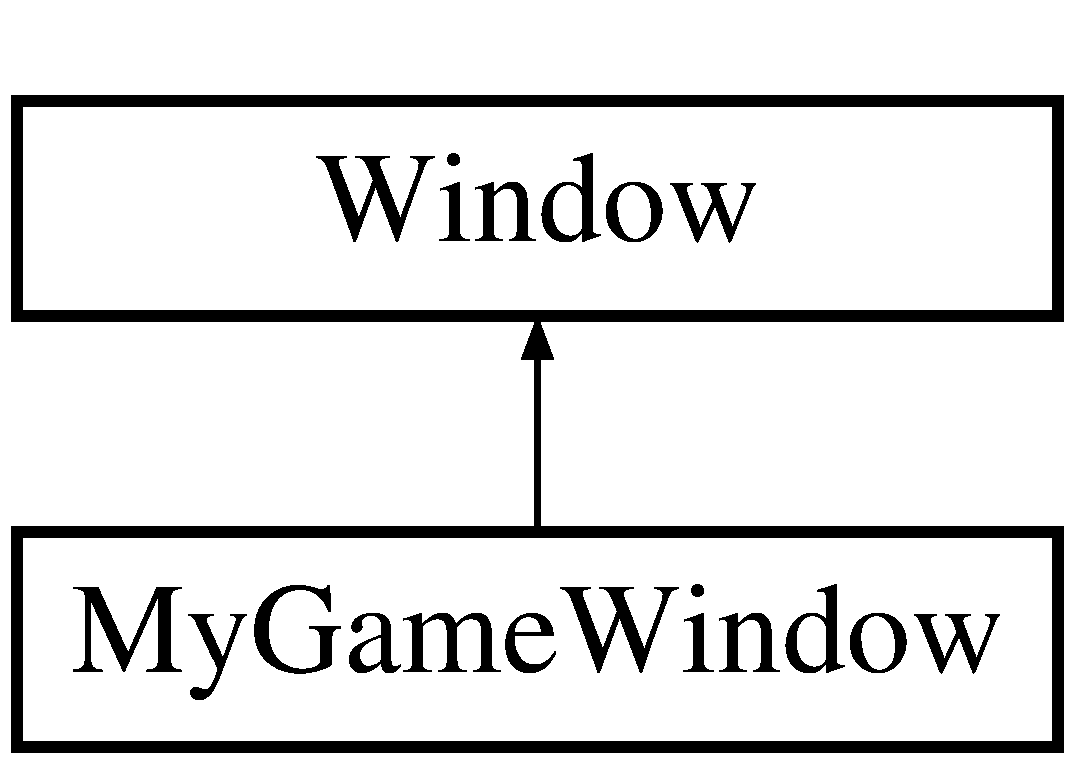
\includegraphics[height=2.000000cm]{classMyGameWindow}
\end{center}
\end{figure}
\subsection*{Public Member Functions}
\begin{DoxyCompactItemize}
\item 
\hypertarget{classMyGameWindow_ac3e84e5b4383f38d08fd22e6d48bb730}{}virtual bool {\bfseries main\+Loop} (S\+D\+L\+\_\+\+Event event, void $\ast$data)\label{classMyGameWindow_ac3e84e5b4383f38d08fd22e6d48bb730}

\item 
\hypertarget{classMyGameWindow_a99600cb93953f642d2fca46c512f1e9a}{}{\bfseries My\+Game\+Window} (std\+::string title, int x, int y, int w, int h)\label{classMyGameWindow_a99600cb93953f642d2fca46c512f1e9a}

\end{DoxyCompactItemize}
\subsection*{Additional Inherited Members}


The documentation for this class was generated from the following file\+:\begin{DoxyCompactItemize}
\item 
/home/batman/code/my\+\_\+git\+\_\+code/yap/src/game/mygame.\+hpp\end{DoxyCompactItemize}

\hypertarget{classPlayer}{}\section{Player Class Reference}
\label{classPlayer}\index{Player@{Player}}
Inheritance diagram for Player\+:\begin{figure}[H]
\begin{center}
\leavevmode
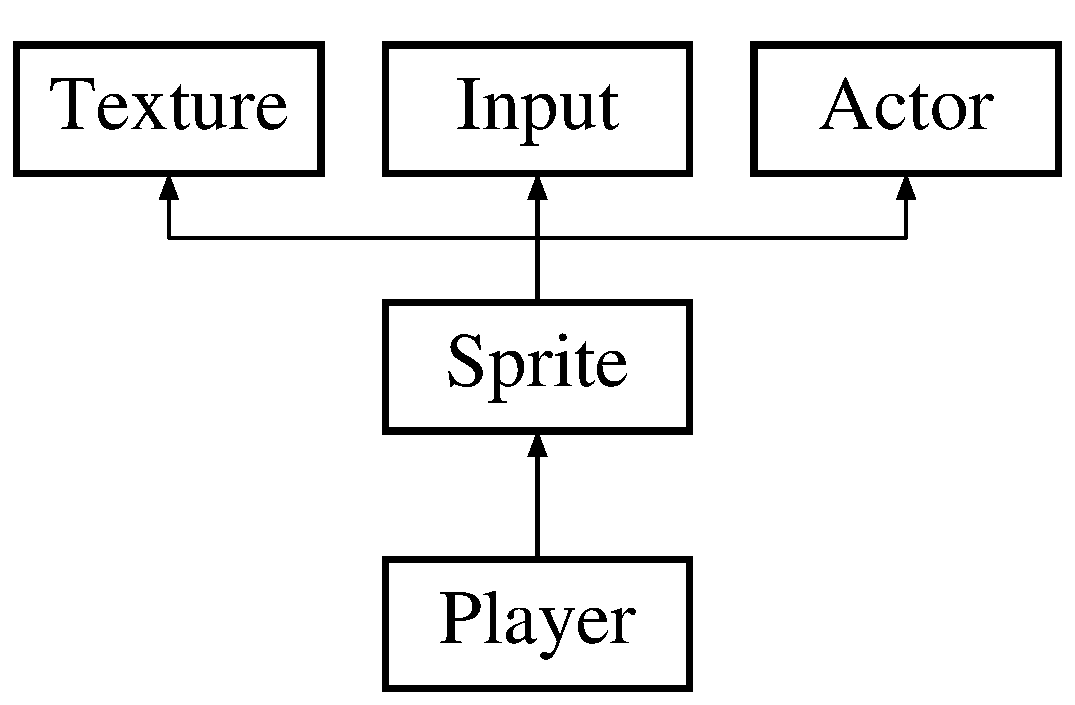
\includegraphics[height=3.000000cm]{classPlayer}
\end{center}
\end{figure}
\subsection*{Public Member Functions}
\begin{DoxyCompactItemize}
\item 
\hypertarget{classPlayer_a1a4c1ee6f4388d60ade10274b551a266}{}{\bfseries Player} (std\+::string texname, cp\+Vect pos, cp\+Vect size, S\+D\+L\+\_\+\+Renderer $\ast$rnd, S\+D\+L\+\_\+\+Window $\ast$window, S\+D\+L\+\_\+\+Event \&ev, bool is\+Dynamic)\label{classPlayer_a1a4c1ee6f4388d60ade10274b551a266}

\item 
\hypertarget{classPlayer_aec1745c553b40fdb8a8d475668ff5dc8}{}virtual void {\bfseries handle\+Events} ()\label{classPlayer_aec1745c553b40fdb8a8d475668ff5dc8}

\item 
\hypertarget{classPlayer_acfbff530f5b4a879ca77241dbcc8d948}{}virtual void {\bfseries update} ()\label{classPlayer_acfbff530f5b4a879ca77241dbcc8d948}

\end{DoxyCompactItemize}
\subsection*{Additional Inherited Members}


The documentation for this class was generated from the following file\+:\begin{DoxyCompactItemize}
\item 
/home/batman/code/my\+\_\+git\+\_\+code/yap/src/gameplay/player.\+hpp\end{DoxyCompactItemize}

\hypertarget{classSprite}{}\section{Sprite Class Reference}
\label{classSprite}\index{Sprite@{Sprite}}
Inheritance diagram for Sprite\+:\begin{figure}[H]
\begin{center}
\leavevmode
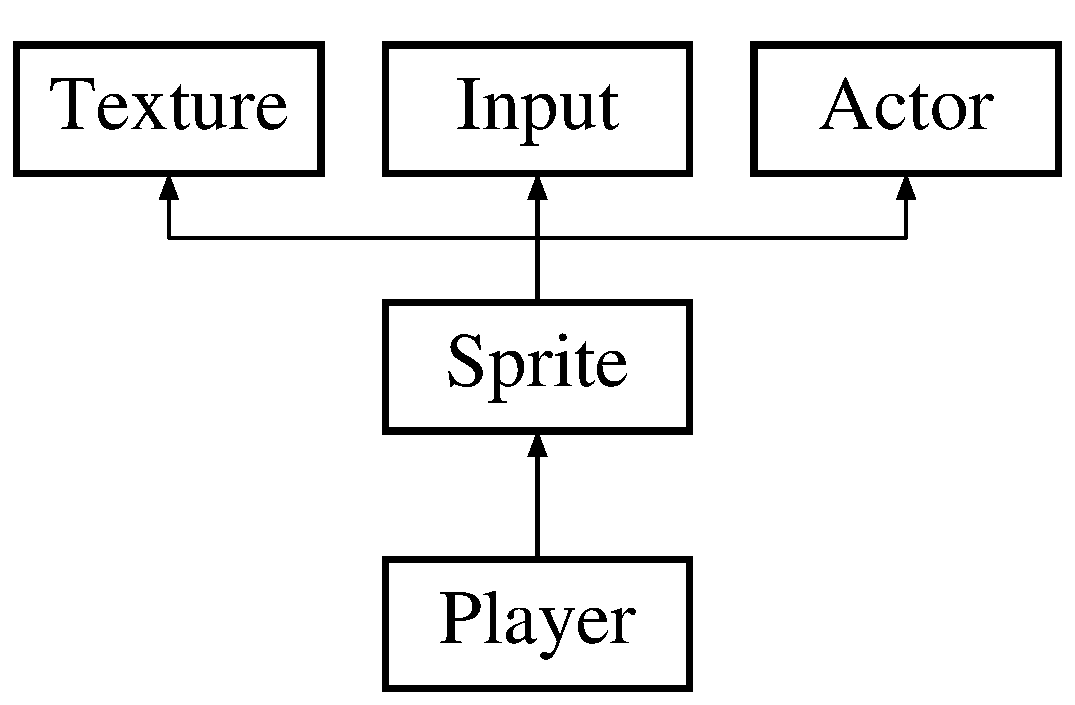
\includegraphics[height=3.000000cm]{classSprite}
\end{center}
\end{figure}
\subsection*{Public Member Functions}
\begin{DoxyCompactItemize}
\item 
\hypertarget{classSprite_a5394486dbe5ce31050782268622ea964}{}{\bfseries Sprite} (std\+::string texname, cp\+Vect pos, cp\+Vect size, S\+D\+L\+\_\+\+Renderer $\ast$rnd, S\+D\+L\+\_\+\+Window $\ast$window, S\+D\+L\+\_\+\+Event \&ev, bool is\+Dynamic)\label{classSprite_a5394486dbe5ce31050782268622ea964}

\item 
\hypertarget{classSprite_a96e2a118c86a5bbcd95c498277f51109}{}virtual void {\bfseries handle\+Events} ()\label{classSprite_a96e2a118c86a5bbcd95c498277f51109}

\end{DoxyCompactItemize}
\subsection*{Additional Inherited Members}


The documentation for this class was generated from the following file\+:\begin{DoxyCompactItemize}
\item 
/home/batman/code/my\+\_\+git\+\_\+code/yap/src/gameplay/sprite.\+hpp\end{DoxyCompactItemize}

\hypertarget{classText}{}\section{Text Class Reference}
\label{classText}\index{Text@{Text}}
\subsection*{Public Member Functions}
\begin{DoxyCompactItemize}
\item 
\hypertarget{classText_a072f1a0f77bf9a4f98e0019164c91e8a}{}{\bfseries Text} (int x, int y, std\+::string txt, T\+T\+F\+\_\+\+Font $\ast$F\+O\+N\+T, int size, S\+D\+L\+\_\+\+Color C\+O\+L\+O\+R, S\+D\+L\+\_\+\+Renderer $\ast$rnd)\label{classText_a072f1a0f77bf9a4f98e0019164c91e8a}

\item 
\hypertarget{classText_a7d35d487d1b61052257473d88392d6fb}{}void {\bfseries update} ()\label{classText_a7d35d487d1b61052257473d88392d6fb}

\item 
\hypertarget{classText_ae0ebbbf31a5913c9ff35ab56155308f6}{}void {\bfseries set\+Text} (std\+::string txt, int size=20)\label{classText_ae0ebbbf31a5913c9ff35ab56155308f6}

\item 
\hypertarget{classText_acaf0220cf5f9c5346570ccad63628e82}{}void {\bfseries set\+Color} (S\+D\+L\+\_\+\+Color C\+O\+L\+O\+R)\label{classText_acaf0220cf5f9c5346570ccad63628e82}

\item 
\hypertarget{classText_a41bde5662e0e3a023166e5b134488bc2}{}std\+::string {\bfseries get\+Text} ()\label{classText_a41bde5662e0e3a023166e5b134488bc2}

\end{DoxyCompactItemize}
\subsection*{Protected Attributes}
\begin{DoxyCompactItemize}
\item 
\hypertarget{classText_aacef942c163c3fdc6258d1aff924d27c}{}std\+::string {\bfseries text}\label{classText_aacef942c163c3fdc6258d1aff924d27c}

\item 
\hypertarget{classText_ac67c9c21854422cb8820f126f749cf16}{}int {\bfseries pt\+Size}\label{classText_ac67c9c21854422cb8820f126f749cf16}

\item 
\hypertarget{classText_ab0f771bd18d8e968f7aaee4a4e26e385}{}S\+D\+L\+\_\+\+Color {\bfseries color}\label{classText_ab0f771bd18d8e968f7aaee4a4e26e385}

\item 
\hypertarget{classText_a5e4a53cb2f8777da607763ccc7c73f2b}{}S\+D\+L\+\_\+\+Texture $\ast$ {\bfseries rendered\+\_\+text}\label{classText_a5e4a53cb2f8777da607763ccc7c73f2b}

\item 
\hypertarget{classText_ae23ac53acb57e760b91c81d8c4aec8c7}{}T\+T\+F\+\_\+\+Font $\ast$ {\bfseries font}\label{classText_ae23ac53acb57e760b91c81d8c4aec8c7}

\item 
\hypertarget{classText_ad26c71bb23e87ed69b9e38210bdde932}{}S\+D\+L\+\_\+\+Renderer $\ast$ {\bfseries renderer}\label{classText_ad26c71bb23e87ed69b9e38210bdde932}

\item 
\hypertarget{classText_a64f890bd55dee40dff17be443d1aa779}{}S\+D\+L\+\_\+\+Rect $\ast$ {\bfseries size}\label{classText_a64f890bd55dee40dff17be443d1aa779}

\end{DoxyCompactItemize}


The documentation for this class was generated from the following file\+:\begin{DoxyCompactItemize}
\item 
/home/batman/code/my\+\_\+git\+\_\+code/yap/src/gfx/text.\+hpp\end{DoxyCompactItemize}

\hypertarget{classTexture}{}\section{Texture Class Reference}
\label{classTexture}\index{Texture@{Texture}}
Inheritance diagram for Texture\+:\begin{figure}[H]
\begin{center}
\leavevmode
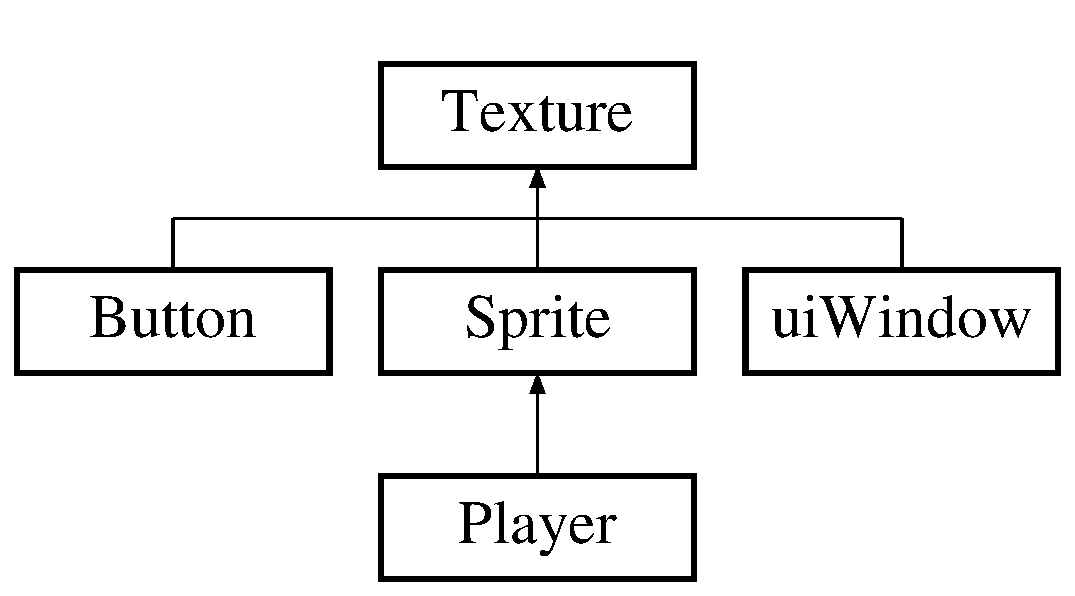
\includegraphics[height=3.000000cm]{classTexture}
\end{center}
\end{figure}
\subsection*{Public Member Functions}
\begin{DoxyCompactItemize}
\item 
\hypertarget{classTexture_a12e9444b8f290a4b70f2afaf86107ad3}{}{\bfseries Texture} (std\+::string texname, int x, int y, S\+D\+L\+\_\+\+Renderer $\ast$rnd, S\+D\+L\+\_\+\+Window $\ast$wind)\label{classTexture_a12e9444b8f290a4b70f2afaf86107ad3}

\item 
\hypertarget{classTexture_aaaee3c61379b8bf4f2ef545eaa232f6a}{}S\+D\+L\+\_\+\+Texture $\ast$ {\bfseries get\+Image} ()\label{classTexture_aaaee3c61379b8bf4f2ef545eaa232f6a}

\item 
\hypertarget{classTexture_ac6ef519f59a0af5ae6004b09af3c7c80}{}std\+::string {\bfseries get\+Title} ()\label{classTexture_ac6ef519f59a0af5ae6004b09af3c7c80}

\item 
\hypertarget{classTexture_ac3b176c8ffb877bac93b769762843e94}{}void {\bfseries set\+Image} (S\+D\+L\+\_\+\+Texture $\ast$img\+\_\+name)\label{classTexture_ac3b176c8ffb877bac93b769762843e94}

\item 
\hypertarget{classTexture_a4fe73d77b591b9609011ccc69d613c81}{}S\+D\+L\+\_\+\+Rect $\ast$ {\bfseries get\+Size} ()\label{classTexture_a4fe73d77b591b9609011ccc69d613c81}

\item 
\hypertarget{classTexture_a457018a962cb9576ed1ab4c13680db8e}{}S\+D\+L\+\_\+\+Renderer $\ast$ {\bfseries get\+Renderer} ()\label{classTexture_a457018a962cb9576ed1ab4c13680db8e}

\item 
\hypertarget{classTexture_a83d747010b0955170ebcd63941e32c20}{}virtual void {\bfseries update} ()\label{classTexture_a83d747010b0955170ebcd63941e32c20}

\end{DoxyCompactItemize}
\subsection*{Protected Attributes}
\begin{DoxyCompactItemize}
\item 
\hypertarget{classTexture_ae939175c09245afc0ab21ad03f0c1d8f}{}S\+D\+L\+\_\+\+Rect $\ast$ {\bfseries size}\label{classTexture_ae939175c09245afc0ab21ad03f0c1d8f}

\item 
\hypertarget{classTexture_aa7452e254b9eef40a4e180f696c712bc}{}S\+D\+L\+\_\+\+Texture $\ast$ {\bfseries tex}\label{classTexture_aa7452e254b9eef40a4e180f696c712bc}

\item 
\hypertarget{classTexture_a0c3be0af7dab3095fe0e6786e83dbd11}{}std\+::string {\bfseries title}\label{classTexture_a0c3be0af7dab3095fe0e6786e83dbd11}

\item 
\hypertarget{classTexture_ad6d227cb6ba9ed5713bfa8b9702e5c20}{}S\+D\+L\+\_\+\+Renderer $\ast$ {\bfseries renderer}\label{classTexture_ad6d227cb6ba9ed5713bfa8b9702e5c20}

\item 
\hypertarget{classTexture_a9c05f0b3afac1695d7c196b9a2103c93}{}S\+D\+L\+\_\+\+Window $\ast$ {\bfseries window}\label{classTexture_a9c05f0b3afac1695d7c196b9a2103c93}

\end{DoxyCompactItemize}


The documentation for this class was generated from the following file\+:\begin{DoxyCompactItemize}
\item 
/home/batman/code/my\+\_\+git\+\_\+code/yap/src/gfx/texture.\+hpp\end{DoxyCompactItemize}

\hypertarget{classuiWindow}{}\section{ui\+Window Class Reference}
\label{classuiWindow}\index{ui\+Window@{ui\+Window}}
Inheritance diagram for ui\+Window\+:\begin{figure}[H]
\begin{center}
\leavevmode
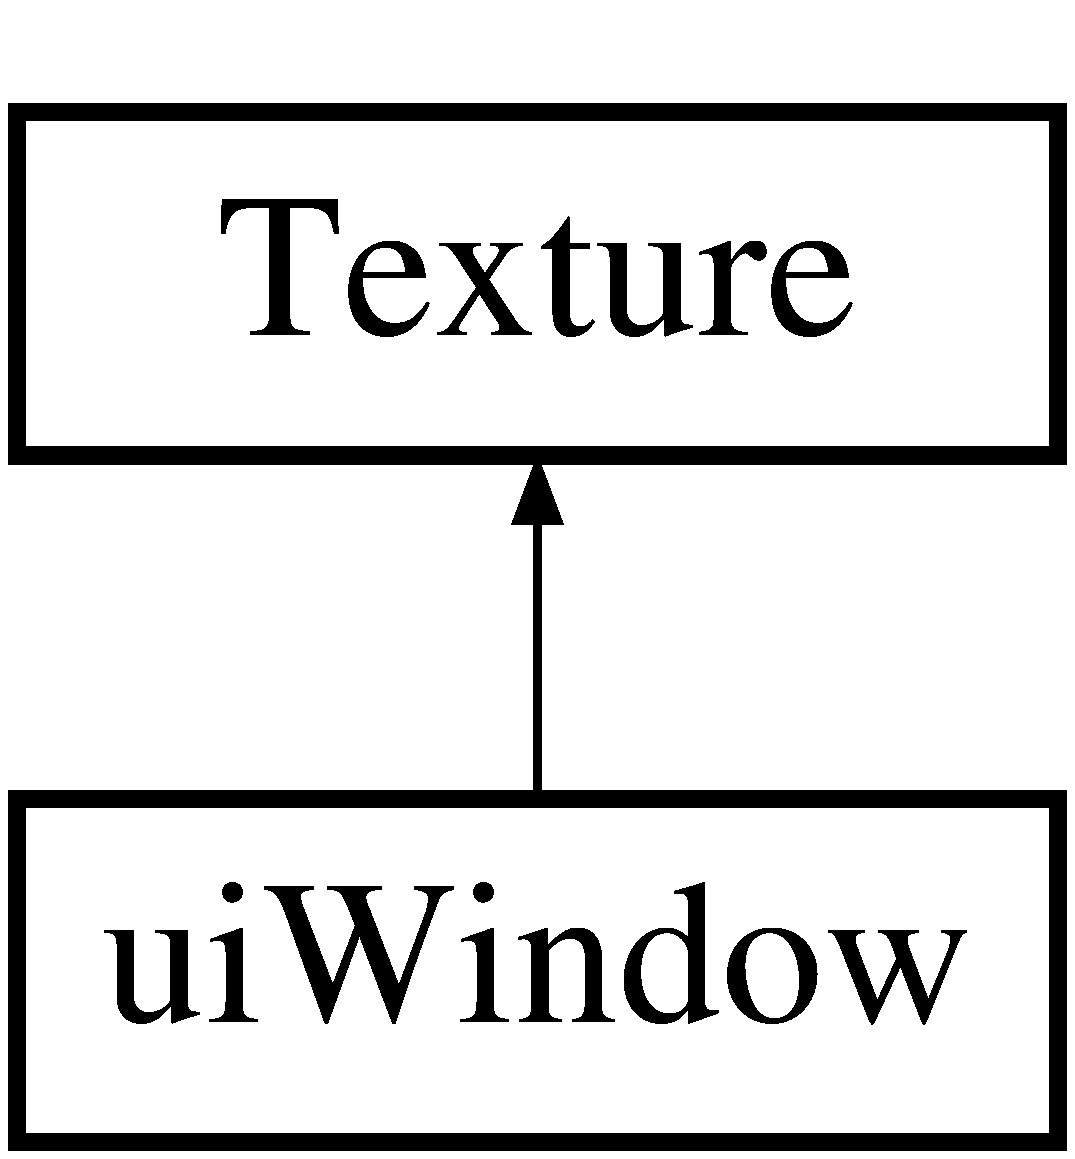
\includegraphics[height=2.000000cm]{classuiWindow}
\end{center}
\end{figure}
\subsection*{Public Member Functions}
\begin{DoxyCompactItemize}
\item 
\hypertarget{classuiWindow_ae3f70599ad9b8b7cbc04897c952c0003}{}{\bfseries ui\+Window} (std\+::string texname, int x, int y, S\+D\+L\+\_\+\+Renderer $\ast$rnd, S\+D\+L\+\_\+\+Window $\ast$window)\label{classuiWindow_ae3f70599ad9b8b7cbc04897c952c0003}

\end{DoxyCompactItemize}
\subsection*{Protected Attributes}
\begin{DoxyCompactItemize}
\item 
\hypertarget{classuiWindow_a059e97109d34fb9e0337ad51bc326bd0}{}std\+::vector$<$ \hyperlink{classButton}{Button} $>$ {\bfseries buttons}\label{classuiWindow_a059e97109d34fb9e0337ad51bc326bd0}

\end{DoxyCompactItemize}


The documentation for this class was generated from the following file\+:\begin{DoxyCompactItemize}
\item 
/home/batman/code/my\+\_\+git\+\_\+code/yap/src/gfx/ui/window.\+hpp\end{DoxyCompactItemize}

\hypertarget{classVelocity}{}\section{Velocity Class Reference}
\label{classVelocity}\index{Velocity@{Velocity}}
\subsection*{Public Member Functions}
\begin{DoxyCompactItemize}
\item 
\hypertarget{classVelocity_ad25d335f5ccd7c24fbe853abee443ff0}{}{\bfseries Velocity} (int xx, int yy)\label{classVelocity_ad25d335f5ccd7c24fbe853abee443ff0}

\item 
\hypertarget{classVelocity_aa16dd3e5db060cbfa0763942b75bb880}{}\hyperlink{classVelocity}{Velocity} {\bfseries operator+} (\hyperlink{classVelocity}{Velocity} rhs)\label{classVelocity_aa16dd3e5db060cbfa0763942b75bb880}

\item 
\hypertarget{classVelocity_a9ce7914dc2557b666127c241041b6354}{}\hyperlink{classVelocity}{Velocity} {\bfseries operator-\/} (\hyperlink{classVelocity}{Velocity} rhs)\label{classVelocity_a9ce7914dc2557b666127c241041b6354}

\item 
\hypertarget{classVelocity_ad2ebf7e97e9820609a6e6dd55e56cc1f}{}void {\bfseries operator+=} (\hyperlink{classVelocity}{Velocity} rhs)\label{classVelocity_ad2ebf7e97e9820609a6e6dd55e56cc1f}

\item 
\hypertarget{classVelocity_a1196064ccbe7f1faa584260dbab50982}{}void {\bfseries operator-\/=} (\hyperlink{classVelocity}{Velocity} rhs)\label{classVelocity_a1196064ccbe7f1faa584260dbab50982}

\end{DoxyCompactItemize}
\subsection*{Public Attributes}
\begin{DoxyCompactItemize}
\item 
\hypertarget{classVelocity_a1286d9d936730167034b2937f1c18b89}{}int {\bfseries x}\label{classVelocity_a1286d9d936730167034b2937f1c18b89}

\item 
\hypertarget{classVelocity_a4b1ae93762efafae20f9a5d8a769a9d4}{}int {\bfseries y}\label{classVelocity_a4b1ae93762efafae20f9a5d8a769a9d4}

\end{DoxyCompactItemize}


The documentation for this class was generated from the following file\+:\begin{DoxyCompactItemize}
\item 
/home/batman/code/my\+\_\+git\+\_\+code/yap/src/common.\+hpp\end{DoxyCompactItemize}

\hypertarget{classWindow}{}\section{Window Class Reference}
\label{classWindow}\index{Window@{Window}}
Inheritance diagram for Window\+:\begin{figure}[H]
\begin{center}
\leavevmode
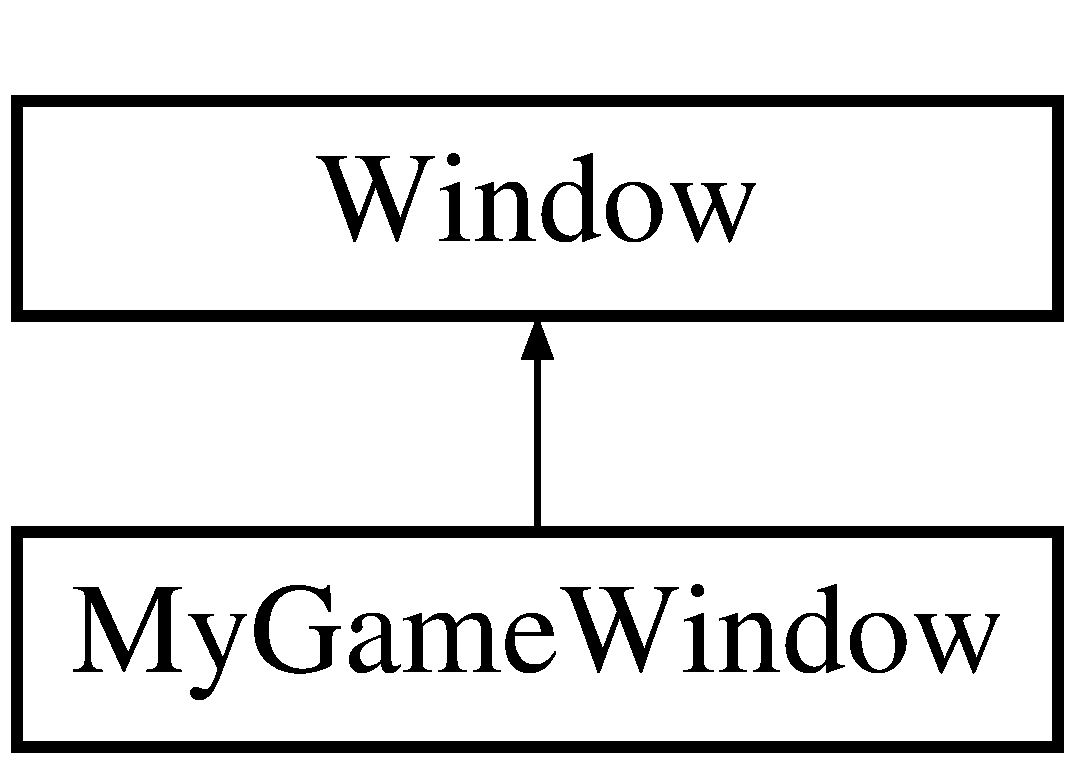
\includegraphics[height=2.000000cm]{classWindow}
\end{center}
\end{figure}
\subsection*{Public Member Functions}
\begin{DoxyCompactItemize}
\item 
\hypertarget{classWindow_a8271c9f315c759d47ec216788ed561e6}{}{\bfseries Window} (std\+::string title, int x, int y, int w, int h)\label{classWindow_a8271c9f315c759d47ec216788ed561e6}

\item 
\hypertarget{classWindow_ad2d885e1e64c00ae20850ee4d1353135}{}S\+D\+L\+\_\+\+Renderer $\ast$ {\bfseries get\+Renderer} ()\label{classWindow_ad2d885e1e64c00ae20850ee4d1353135}

\item 
\hypertarget{classWindow_a58daf43e03ac44a5685a2208faf3f53f}{}S\+D\+L\+\_\+\+Window $\ast$ {\bfseries get\+Window} ()\label{classWindow_a58daf43e03ac44a5685a2208faf3f53f}

\item 
\hypertarget{classWindow_ac8cff5784b0507a91111281c62c9b5c7}{}virtual bool {\bfseries main\+Loop} (S\+D\+L\+\_\+\+Event event, void $\ast$data)\label{classWindow_ac8cff5784b0507a91111281c62c9b5c7}

\item 
\hypertarget{classWindow_a5401a83e70b84e03e84eb07ef9e6e894}{}bool {\bfseries execute} (S\+D\+L\+\_\+\+Event event, void $\ast$data)\label{classWindow_a5401a83e70b84e03e84eb07ef9e6e894}

\end{DoxyCompactItemize}
\subsection*{Protected Attributes}
\begin{DoxyCompactItemize}
\item 
\hypertarget{classWindow_a2b52309ef359b6392454a3bb57398b5d}{}S\+D\+L\+\_\+\+Renderer $\ast$ {\bfseries renderer}\label{classWindow_a2b52309ef359b6392454a3bb57398b5d}

\item 
\hypertarget{classWindow_ae39a7755a5a6ab74bcbdbe3e2e206820}{}S\+D\+L\+\_\+\+Window $\ast$ {\bfseries window}\label{classWindow_ae39a7755a5a6ab74bcbdbe3e2e206820}

\item 
\hypertarget{classWindow_a9a521dcf64e0fc3c4d7f16388fcfca1f}{}int {\bfseries window\+\_\+height}\label{classWindow_a9a521dcf64e0fc3c4d7f16388fcfca1f}

\item 
\hypertarget{classWindow_ac81447b26708f67b69c07e76637d6ecd}{}int {\bfseries window\+\_\+width}\label{classWindow_ac81447b26708f67b69c07e76637d6ecd}

\item 
\hypertarget{classWindow_aa083beca8982ad4445e6047d6f6c7d7b}{}bool {\bfseries done}\label{classWindow_aa083beca8982ad4445e6047d6f6c7d7b}

\end{DoxyCompactItemize}


The documentation for this class was generated from the following file\+:\begin{DoxyCompactItemize}
\item 
/home/batman/code/my\+\_\+git\+\_\+code/yap/src/gfx/ui/window.\+hpp\end{DoxyCompactItemize}

\hypertarget{classWorld}{}\section{World Class Reference}
\label{classWorld}\index{World@{World}}
\subsection*{Public Member Functions}
\begin{DoxyCompactItemize}
\item 
\hypertarget{classWorld_afd25e14cb9229826064e6dc9a372d688}{}{\bfseries World} (cp\+Vect gravity, cp\+Float time)\label{classWorld_afd25e14cb9229826064e6dc9a372d688}

\item 
\hypertarget{classWorld_ac6c94c5ac13d057c6748cc9feb03d849}{}cp\+Space $\ast$ {\bfseries get} ()\label{classWorld_ac6c94c5ac13d057c6748cc9feb03d849}

\item 
\hypertarget{classWorld_ae69934936f105df69f4fbaf9d7e4be6b}{}virtual void {\bfseries update} ()\label{classWorld_ae69934936f105df69f4fbaf9d7e4be6b}

\item 
\hypertarget{classWorld_a41f336246fda93567233e6441c800433}{}void {\bfseries attach\+Actor} (\hyperlink{classActor}{Actor} $\ast$actor)\label{classWorld_a41f336246fda93567233e6441c800433}

\end{DoxyCompactItemize}
\subsection*{Protected Attributes}
\begin{DoxyCompactItemize}
\item 
\hypertarget{classWorld_a484d43ac4b72629d4d32b8eaa51f707e}{}cp\+Vect {\bfseries grav}\label{classWorld_a484d43ac4b72629d4d32b8eaa51f707e}

\item 
\hypertarget{classWorld_a4fb8abef966c6d9750e75ffafa36566e}{}cp\+Space $\ast$ {\bfseries pworld}\label{classWorld_a4fb8abef966c6d9750e75ffafa36566e}

\item 
\hypertarget{classWorld_a0e13789989b30b7314e6e376d600bd24}{}cp\+Float {\bfseries timestep}\label{classWorld_a0e13789989b30b7314e6e376d600bd24}

\item 
\hypertarget{classWorld_aea7c237000a3b38c8e2d1c56202ab649}{}std\+::vector$<$ \hyperlink{classActor}{Actor} $\ast$ $>$ {\bfseries actors}\label{classWorld_aea7c237000a3b38c8e2d1c56202ab649}

\end{DoxyCompactItemize}


The documentation for this class was generated from the following file\+:\begin{DoxyCompactItemize}
\item 
/home/batman/code/my\+\_\+git\+\_\+code/yap/src/physics/world.\+hpp\end{DoxyCompactItemize}

%--- End generated contents ---

% Index
\backmatter
\newpage
\phantomsection
\clearemptydoublepage
\addcontentsline{toc}{chapter}{Index}
\printindex

\end{document}
